\documentclass[tikz,border=5pt]{standalone}
\usepackage{fontspec}
\setmainfont{Times New Roman}
\usepackage{unicode-math}
\setmathfont{Cambria Math}
\usetikzlibrary{shapes.geometric,positioning,fit,backgrounds,arrows.meta,calc}

\begin{document}
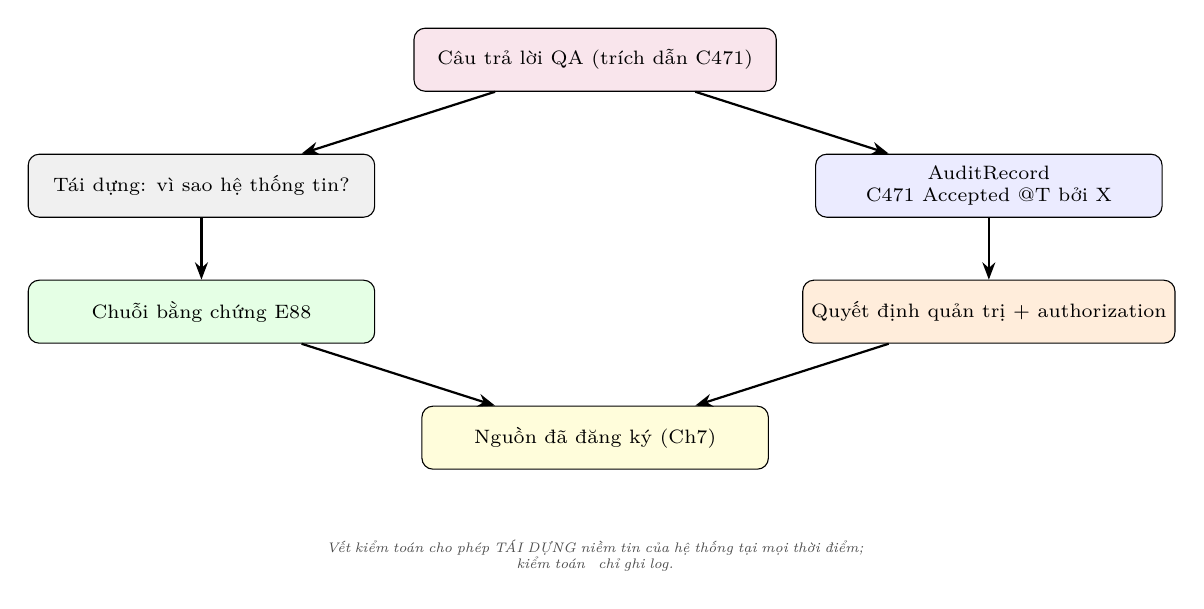
\begin{tikzpicture}[
  box/.style={rectangle, draw, rounded corners, align=center, font=\scriptsize, inner sep=3pt},
  arrow/.style={-{Stealth[length=2.2mm]}, thick},
  label/.style={font=\tiny\itshape, text=gray!60!black},
]

% === AUDIT TRAIL REPLAY ===
\node[box, fill=purple!10, minimum width=4.6cm, minimum height=0.8cm] (ans) at (0, 4.4) {Câu trả lời QA (trích dẫn C471)};

\node[box, fill=gray!12, minimum width=4.4cm, minimum height=0.8cm] (reve) at (-5.0, 2.8) {Tái dựng: vì sao hệ thống tin?};
\node[box, fill=blue!8, minimum width=4.4cm, minimum height=0.8cm] (audr) at (5.0, 2.8) {AuditRecord\\C471 Accepted @T bởi X};

\node[box, fill=green!10, minimum width=4.4cm, minimum height=0.8cm] (ev) at (-5.0, 1.2) {Chuỗi bằng chứng E88};
\node[box, fill=orange!14, minimum width=4.4cm, minimum height=0.8cm] (gov) at (5.0, 1.2) {Quyết định quản trị + authorization};

\node[box, fill=yellow!14, minimum width=4.4cm, minimum height=0.8cm] (src) at (0, -0.4) {Nguồn đã đăng ký (Ch7)};

\draw[arrow] (ans) -- (reve);
\draw[arrow] (ans) -- (audr);
\draw[arrow] (reve) -- (ev);
\draw[arrow] (audr) -- (gov);
\draw[arrow] (ev) -- (src);
\draw[arrow] (gov) -- (src);

\node[label, align=center, text width=11cm] at (0, -1.9)
  {Vết kiểm toán cho phép TÁI DỰNG niềm tin của hệ thống tại mọi thời điểm;\\kiểm toán ≠ chỉ ghi log.};
\end{tikzpicture}
\end{document}